\documentclass[12pt,oneside,a4paper]{article}

\usepackage[backend=biber,style=numeric]{biblatex}
\usepackage{xcolor}
\usepackage{todonotes}
\usepackage{amsmath}
\usepackage{multicol}
\usepackage{caption}
\usepackage{hyperref}
\usepackage{graphicx}
\usepackage{listings}
\lstset{
	frame=top,frame=bottom,
	language=C,
	basicstyle=\small\normalfont,
	xleftmargin=\parindent,
	keywordstyle=\color{green!40!black},
	%  commentstyle=\itshape\color{purple!40!black},
	%  identifierstyle=\color{blue},
	%  stringstyle=\color{orange},
	morekeywords={in, globaldata, procedure, input, output, behavior, end, XOR, NOT, AND}, % keyword to highlight
	%  captionpos=t,
	tabsize=2,
	numbers=left,
	stepnumber=1,                   % the step between two line-numbers.        
	numbersep=5pt,
	framexleftmargin=10pt,
	title=\lstname,
	captionpos=t,
	showspaces=false,
}
\DeclareCaptionFormat{listing}{\rule{\dimexpr\textwidth\relax}{0.4pt}\par\vskip1pt#1#2#3}
\captionsetup[lstlisting]{format=listing,singlelinecheck=false, margin=0pt,labelsep=space,labelfont=bf}

\usepackage{booktabs}
\usepackage[noabbrev,capitalise]{cleveref}
\crefname{listing}{algorithm}{algorithms}
\Crefname{listing}{Algorithm}{Algorithms}
\renewcommand\lstlistingname{Algorithm}
\def\lstlistingcrefname{Algorithm}
\usepackage{url}

\addbibresource{biblio.bib}

\title{\textbf{Alimentazione \& Psicologia}}

\author{Manuel Colombo}

\date{2023}

\begin{document}


\begin{titlepage}
	\centering
	\clearpage
	\maketitle
	\thispagestyle{empty}
	\vspace*{1cm}
	\vfill
	\centering
	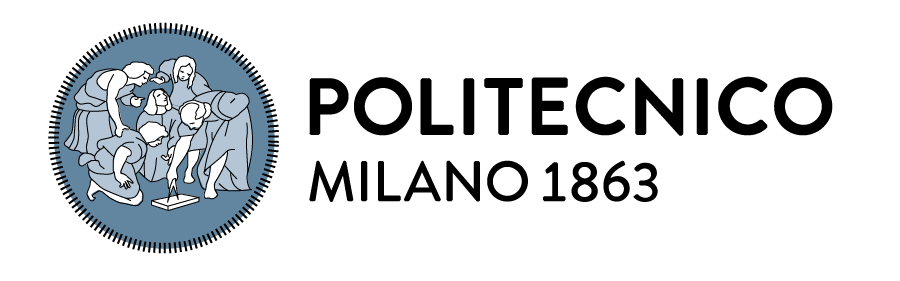
\includegraphics{logo_polimi.png}
\includegraphics{logo_NECST.png}
\end{titlepage}


\section{Introduzione} \label{sec:intro}
Questo articolo si propone di esplorare l'importante interazione tra cibo e psicologia, concentrandosi sull'esperienza del cibo e il suo impatto sulla psicologia individuale e collettiva. Il cibo non è solo una fonte di nutrimento, ma influenza anche il nostro benessere emotivo, le emozioni e i comportamenti. Comprendere questa interazione può fornire preziose informazioni per promuovere una relazione sana con il cibo e migliorare la qualità della vita. Attraverso una revisione della letteratura e l'analisi di studi pertinenti, questo articolo si propone di esaminare i vari aspetti dell'esperienza del cibo e il modo in cui influenzano la psicologia umana. 

\section{Alimentazione e benessere psicologico } \label{sec:aleben}
I fattori psicologici legati al cibo possono influenzare significativamente le nostre abitudini alimentari e il nostro benessere complessivo. Un comportamento comune è mangiare mentre si svolge un'altra attività, come studiare. Questo indica che spesso siamo impegnati in troppe cose contemporaneamente, sovraccaricando la mente e il corpo. Tuttavia, sovraccaricarsi con troppe attività non è salutare per la nostra salute e il nostro benessere. Mangiare distrattamente può ridurre la consapevolezza di ciò che mangiamo e dei segnali di sazietà, contribuendo all'aumento di peso e ad abitudini alimentari poco salutari. È importante dedicare momenti tranquilli e consapevoli al pasto, evitando sovraccarichi di attività simultanee, per promuovere una relazione più equilibrata e salutare con il cibo. 

Tuttavia, il momento del pasto condiviso può contribuire a ridurre lo stress, migliorare l'umore e aumentare la soddisfazione complessiva della vita. Approfondire i benefici di mangiare in compagnia può fornire preziose informazioni per incoraggiare il mantenimento di relazioni sociali salutari e promuovere una migliore qualità della vita. 
\begin{figure}[h]
    \centering
    
\includegraphics[width=.9\textwidth]{cibo1.png}
    \label{fig:my_label}
\end{figure}

\section{Fame emotiva } \label{sec:famem}
La fame emotiva si verifica quando il cibo viene utilizzato come una forma di conforto o gratificazione per alleviare emozioni spiacevoli come l'ansia, la rabbia o la tristezza. Spesso, questo comportamento avviene in modo inconsapevole o automatico, senza che la persona se ne renda conto. 

Il processo della fame emotiva può essere descritto come un ciclo che inizia con l'esperienza di un'emozione negativa. Questa emozione crea il bisogno di conforto, che si traduce in un impulso a mangiare come modo per sentirsi temporaneamente meglio. Mangiare porta a una sensazione di benessere momentaneo, ma contemporaneamente aumenta il bisogno di sentirsi ancora "meglio". Alla fine, la persona può sperimentare un senso di colpa o vergogna per aver mangiato in modo eccessivo o poco salutare. 

Le emozioni svolgono un ruolo importante nella vita di un individuo, aiutandolo a comprendere l'ambiente circostante e a definire i comportamenti più adattivi e funzionali. Tuttavia, le emozioni possono diventare problematiche quando superano i livelli appropriati in termini di intensità o durata. Inoltre, se le emozioni si manifestano in contesti inadeguati o in modi imprevedibili, possono creare difficoltà e disagio nella vita di una persona. La fame emotiva può essere considerata una risposta disfunzionale alle emozioni, poiché il cibo diventa un mezzo per gestire o sopprimere le emozioni spiacevoli anziché affrontarle in modo più sano ed efficace. Affrontare la fame emotiva richiede una maggiore consapevolezza delle proprie emozioni e l'adozione di strategie alternative per gestirle, come la pratica di tecniche di rilassamento, l'esercizio fisico o il ricorso al supporto sociale. 
\begin{figure}[h]
    \centering
    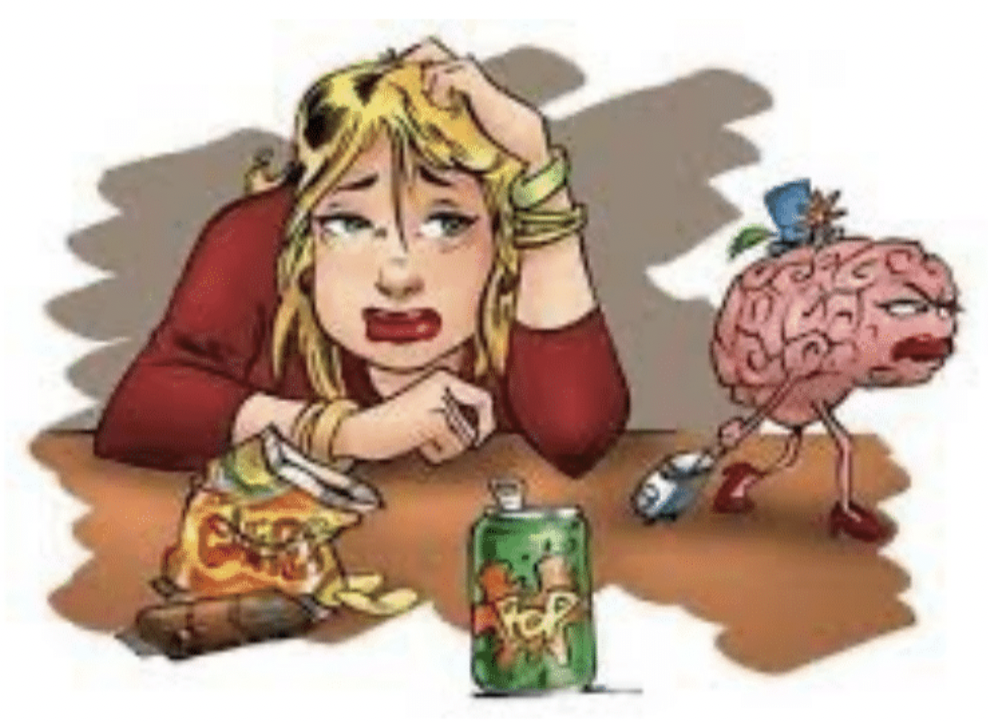
\includegraphics[width=.7\textwidth]{fame.png}
    \label{fig:my_label}
\end{figure}

\section{Fame emotiva vs fame fisica } \label{sec:emfis}
La distinzione tra fame emotiva e fame fisica è di fondamentale importanza. La fame fisica si manifesta gradualmente nel corpo, è una sensazione che può essere attesa e viene soddisfatta gradualmente con il cibo. Non è accompagnata da sensi di colpa o vergogna. È semplicemente una risposta biologica alla necessità di nutrimento. 

D'altra parte, la fame emotiva arriva all'improvviso e richiede una soddisfazione immediata. Non è legata a una vera necessità fisiologica, ma piuttosto a una risposta alle emozioni spiacevoli o a uno stato mentale negativo. Può essere scatenata da stress, noia, solitudine o altre emozioni difficili da affrontare. Quando si sperimenta la fame emotiva, spesso si prova un senso di colpa, vergogna e talvolta una sensazione di sconfitta per non essere in grado di gestire le emozioni in modo diverso. 

\section{Trappole alimentari delle gratificazioni immediate } \label{sec:trap}
La capacità di controllare i comportamenti impulsivi di fronte a emozioni negative è cruciale per mantenere relazioni sane e gestire efficacemente lo stress. Tuttavia, per raggiungere questo obiettivo, è importante evitare determinate azioni suggerite nell'elenco puntato successivo. Ad esempio, nel caso della noia, è consigliabile fare scelte salutari come consumare frutta anziché cedere all'impulso di mangiare cibi poco salutari. Per quanto riguarda l'ansia, è preferibile soddisfare e calmare il corpo con alternative migliori rispetto al consumo di sale e zucchero, che possono creare dipendenza e non affrontare realmente le cause dell'ansia. Inoltre, per gestire la rabbia, è consigliabile cercare strategie alternative, invece di sgranocchiare cibo salato che può portare solo a un sollievo temporaneo. Infine, nel caso della tristezza, è importante considerare alternative più sane all'uso di zucchero e cioccolato come "antidepressivi naturali", concentrandosi invece su metodi di affrontamento che promuovano il benessere generale. 

\section{Conclusioni} \label{sec:concl}
In conclusione, l'interazione tra cibo e psicologia è un elemento importante da considerare per migliorare la qualità della vita. Comprendere come il cibo influenzi le nostre emozioni, comportamenti e benessere psicologico può aiutarci a sviluppare una relazione più equilibrata con il cibo. Evitare di mangiare in modo distratto, dedicare momenti di tranquillità al pasto e condividere i pasti con gli altri può favorire il benessere emotivo. Inoltre, riconoscere la differenza tra fame emotiva e fame fisica può aiutare a gestire le emozioni in modo più sano. Sviluppare alternative salutari alle gratificazioni immediate può promuovere un benessere generale e una gestione efficace dello stress. 


\newpage
\title{\textbf{Bibliografia}} \\
\begin{itemize}
\item Meeting NecstCAMP del 23/11/2022 tenuto dalle dottoresse Silvia Danna e Gloria Romeo
\item Meeting NecstCAMP del 25/03/2023 tenuto dalle dottoresse Silvia Danna e Gloria Romeo
\end{itemize}

\end{document}


